In der Bildverarbeitung kann ein gegebenes Signal häufig nur durch eine
unstetige Funktion dargestellt werden. Deshalb stellt sich zunächst die Frage,
welcher Funktionenraum zum Beschreiben dieser Signale geeignet ist.

Sei $\Omega\subset\Rbb^2$ ein polygonal berandetes Lipschitz-Gebiet und
$g:\Omega\to \Rbb$ stelle ein gegebenes Signal auf $\Omega$ dar. 
Das Signal $g$ könnte im Sobolev-Raum $W^{1,1}(\Omega)$ vermutet werden, da
Elemente dieses Raums im Allgemeinen nicht stetig sein müssen. 
Allerdings lassen Sobolev-Funktionen die oftmals benötigten Sprünge über
Teilmengen niedrigerer Dimension von $\Omega$ nicht zu
\cite[297]{Bar15}.
Dieses Problem kann gelöst werden, indem der Raum der Funktionen von
beschränkter Variation $\BV(\Omega)$ betrachtet wird. 
Dieser ist eine echte Obermenge von $W^{1,1}(\Omega)$ und hat sich als geeignet
für die Modellierung von Signalen in der Bildverarbeitung und weitere
Anwendungen erwiesen (cf.\ \cites[393]{ABM14}[42]{AK06}[297]{Bar15}[S. 1
f.]{Bra98}).

Eine mögliche Problemstellung in der Bildverarbeitung ist die 
Rauschunterdrü\-ckung, das heißt der Versuch unerwünschtes Rauschen in einem
Signal zu verringern.
In \cite{ROF92} beschrieben Rudin, Osher und Fatemi 1992 das heute als
ROF-Modell bekannte Minimierungsproblem dafür (cf.\
\cites[1217]{Bar15a}[132]{CP10}[S. 74 f.]{Get12}).
Dabei ist für das gegebene Signal $g\in L^2(\Omega)$ und 
eine Funktion $v\in\BV(\Omega)\cap L^2(\Omega)$ die Minimierung
der Summe der zwei folgenden Terme relevant.
Der erste Term ist die
Seminorm
\begin{align*}
  |v|_{\BV(\Omega)}
  \coloneqq
  \sup_{\substack{\phi\in C^\infty_0(\Omega;\Rbb^2)\\
  |\phi|\leq 1}}\int_\Omega v\Div (\phi)\dx
  <
  \infty.
\end{align*}
von $v$ auf $\BV(\Omega)$ \cite[1162]{Bar12}. Diese entspricht der
totalen Variation der distributionellen Ableitung $Dv$ von $v$ und
ihre Minimierung verhindert Oszillationen in der Lösung, lässt aber
Unstetigkeiten zu \cite[72]{Get12}.
Außerdem stimmt diese, falls $v\in W^{1,1}(\Omega)$, mit der Seminorm auf
$W^{1,1}(\Omega)$ überein. 
Der zweite Term $\Vert v-g\Vert_{L^2(\Omega)}^2$ misst den Abstand von $v$ und
$g$ in $L^2(\Omega)$. 
Die Minimierung dieses Terms bewirkt, dass die Lösung dem Eingangssignal
ähnelt.
Mit diesen Termen und mit einen positiven Parameter
$\alpha\in\Rbb_+$, der das Verhältnis zwischen Rauschverminderung und
Ähnlichkeit der Lösung zum Eingangssignal gewichtet, sucht das ROF-Modell
eine Funktion $u\in\BV(\Omega)\cap L^2(\Omega)$, die das Funktional
\begin{align}
  \label{eq:rofModel}
  I(v)\coloneqq |v|_{\BV(\Omega)}+\frac{\alpha}{2}\Vert
  v-g\Vert_{L^2(\Omega)}^2
\end{align}
unter allen $v\in\BV(\Omega)\cap L^2(\Omega)$ minimiert.
Wird hierbei $\alpha$ zu klein gewählt, führt das zu einer zu stark
geglätteten, verwaschen aussehenden Lösung, zu sehen zum Beispiel in den
Abbildungen \ref{fig:snr10alpha100} und \ref{fig:snr10alpha1000}. 
Wird andererseits $\alpha$ zu groß gewählt, ist die Verminderung des Rauschens
im Vergleich zum Eingangssignal $g$ nur gering, zu sehen zum Beispiel in den
Abbildungen \ref{fig:snr10alpha5000} und \ref{fig:snr10alpha10000}.
Für weitere Details und Referenzen zur Rauschunterdrückung und zur Wahl von
$\alpha$ siehe \cite{Get12}.

Zur numerischen Behandlung dieses Problems gibt es bereits einige Ansätze in 
der Literatur. 
Dazu gehören die Regularisierung der Seminorm $|\bullet|_{\BV(\Omega)}$, indem
die Betragsfunktion $|\bullet|$ durch eine stetig differenzierbare
Approximation $|\bullet|_\varepsilon$ ersetzt wird, und die Nutzung von höheren
Ableitungen in der Definition von $|\bullet|_{\BV(\Omega)}$.
Vor- und Nachteile dieser Ansätze und entsprechende Referenzen werden in
\cite[1165]{Bar12} zusammengefasst. 
Außerdem wird ebenda auf Arbeiten verwiesen, in denen verschieden iterative
Lösungsmethoden für das ROF-Modellproblem diskutiert werden.
Professor Bartels untersucht in \cite[Kapitel 10.2]{Bar15} eine
$W^{1,1}$-konforme Diskretisierung des ROF-Modells mit der
Courant-Finite-Elemente-Methode. 
Zur numerischen Lösung dieser diskreten Formulierung nutzt er eine
primale-duale Iteration, welche durch Betachtung der primalen und der dualen
Formulierung des Minimierungsproblems motiviert ist.
Eine Regularisierung oder die Nutzung höherer Ableitungen für die
$\BV$-Seminorm werden dabei nicht benötigt.

In dieser Arbeit möchte wir die Anwendung dieser primalen-dualen Iteration auf
eine nichtkonforme Formulierung des ROF-Modells und einer Diskretisierung
mit der Crouzeix\--Raviart\--Finite\--Elemente\--Methode untersuchen.
Dabei nutzen wir einen von Professor Carstensen zur Verfügung gestellten
Verfeinerungsindikator, um die Iteration im Solve-Schritt der AFEM-Routine
aus \Cref{fig:afemLoop} nutzen zu können. 
Außerdem erlaubt uns die nichtkonforme Formulierung die Betrachtung einer
garantierten unteren Energieschranke, welche ebenfalls von Professor Carstensen
zur Verfügung gestellt wurde.
Die Implementierung des adaptiven Algorithmus basiert auf dem
Matlab-Soft\-ware\-pa\-ket AFEM \cite{Car09}. 

Abschließend sei angemerkt, dass wir folgende, leicht andere Formulierung des 
ROF-Modells betrachten. 
Wir minimieren das Funktional
\begin{align*}
  E(v)\coloneqq \frac{\alpha}{2}\Vert v\Vert_{L^2(\Omega)}^2 + |v|_{\BV(\Omega)}
  +\Vert v\Vert_{L^1(\partial\Omega)}-\int_\Omega fv\dx
\end{align*}
unter allen $v\in\BV(\Omega)\cap L^2(\Omega)$.
Dabei ist der Term  $\Vert v\Vert_{L^1(\partial\Omega)}$ durch den Spursatz für
\BV-Funktionen \cite[S. 400, Theorem 10.2.1]{ABM14} wohldefiniert und seine
Minimierung modelliert homogene Randdaten.
Für $f = \alpha g$ und alle $v\in \BV(\Omega)\cap L^2(\Omega)$ gilt dann $I(v)
= E(v) - \Vert v\Vert_{L^1(\partial \Omega)}+ \frac{\alpha}{2}\Vert
g\Vert_{L^2(\Omega)}^2$. 
Der Zusammenhang mit dem ROF-Modell ist, aufgrund der Konstanz des Terms
$\frac{\alpha}{2}\Vert g\Vert_{L^2(\Omega)}^2$, folglich, dass die Funktionale
$E$ und $I$ die gleichen Minimierer in $\left\{v\in\BV(\Omega)\cap
L^2(\Omega)\mid \Vert v\Vert_{L^1(\partial\Omega)}=0\right\}$ besitzen.

Die Struktur dieser Arbeit ist wie folgt.
Nachdem in \Cref{chap:theoreticalBasics} zunächst die Notationen eingeführt und
die theoretischen Grundlagen aus der Optimierung und zu den Funktionen
beschränkter Variation zusammengetragen wurden, wird in
\Cref{chap:continuousProblem} bewiesen, dass für unsere Formulierung des
ROF-Modells ein eindeutiger Minimierer existiert.
Anschließend folgt in \Cref{chap:discreteProblem} die nichtkonforme
Formulierung und Diskretisierung des Minimierungsproblems. 
Mithilfe der Sattelpunktsformulierung des diskreten Problems werden äquivalente
Charakterisierungen, Existenz und Eindeutigkeit für den diskreten Minimierer
bewiesen. Außerdem werden die zu untersuchenden Konvergenzraten, der
Verfeinerungsindikator und die garantierte untere Energieschranke aufgeführt.
In \Cref{chap:algorithm} wird die primale-duale Iteration formuliert und
bewiesen, dass diese gegen den diskreten Minimierer konvergiert. 
Es folgen in \Cref{chap:implementation} Hinweise zur Benutzung des Programms
und Details zur Implementierung des Algorithmus und schließlich in
\Cref{chap:experiments} die Darstellung der Experimente und deren Auswertung in
\Cref{chap:review}.

\newpage
\begin{figure}[!ht]
  \centering
  \begin{subfigure}[b]{.4\linewidth}
    \caption{Originalbild}
    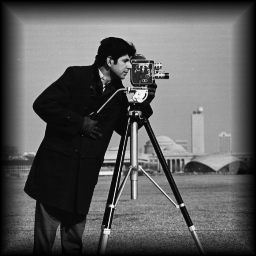
\includegraphics[width=\linewidth]{pictures/introBeta/cameraman.png}
    \label{fig:camerman}
  \end{subfigure}
  \quad
  \begin{subfigure}[b]{.4\linewidth}
    \caption{Originalbild mit AWGN}
    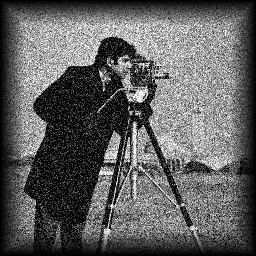
\includegraphics[width=\linewidth]{pictures/introBeta/snr10.png}
    \label{fig:camermanSNR10}
  \end{subfigure}

  \begin{subfigure}{.3\linewidth}
    \caption{$\alpha=100$}
    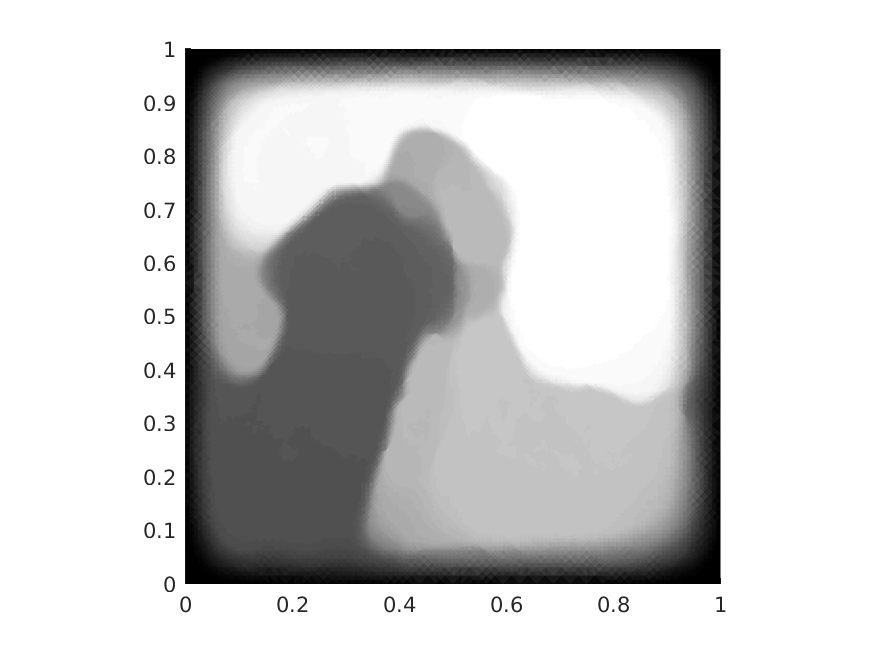
\includegraphics[trim = 60 20 60 20, clip, width=\linewidth]
      {pictures/introBeta/snr10/00100.png}
    \label{fig:snr10alpha100}
  \end{subfigure}
  \begin{subfigure}{.3\linewidth}
    \caption{$\alpha=1000$}
    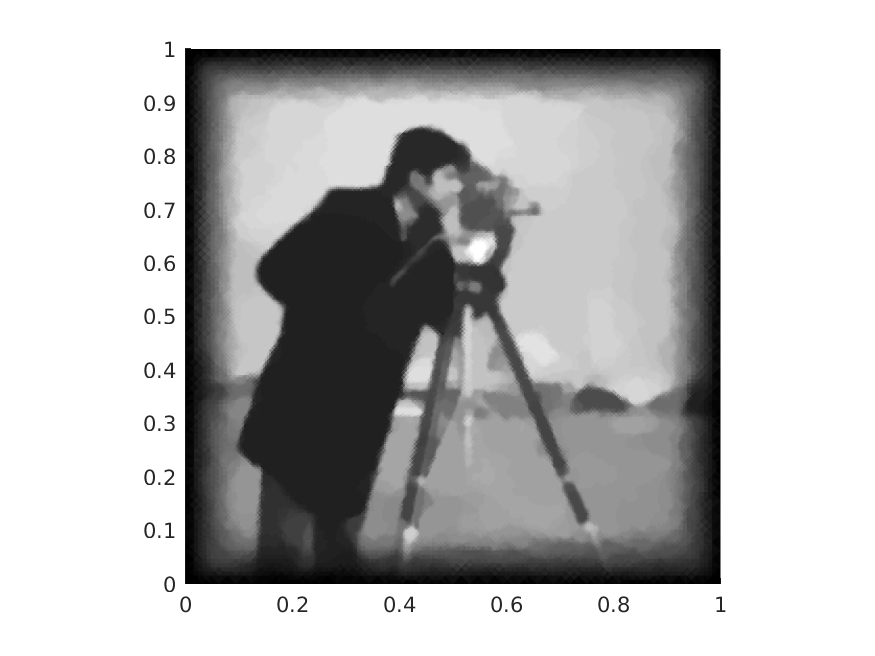
\includegraphics[trim = 60 20 60 20, clip, width=\linewidth]
      {pictures/introBeta/snr10/01000.png}
    \label{fig:snr10alpha1000}
  \end{subfigure}
  \begin{subfigure}{.3\linewidth}
    \caption{$\alpha=2500$}
    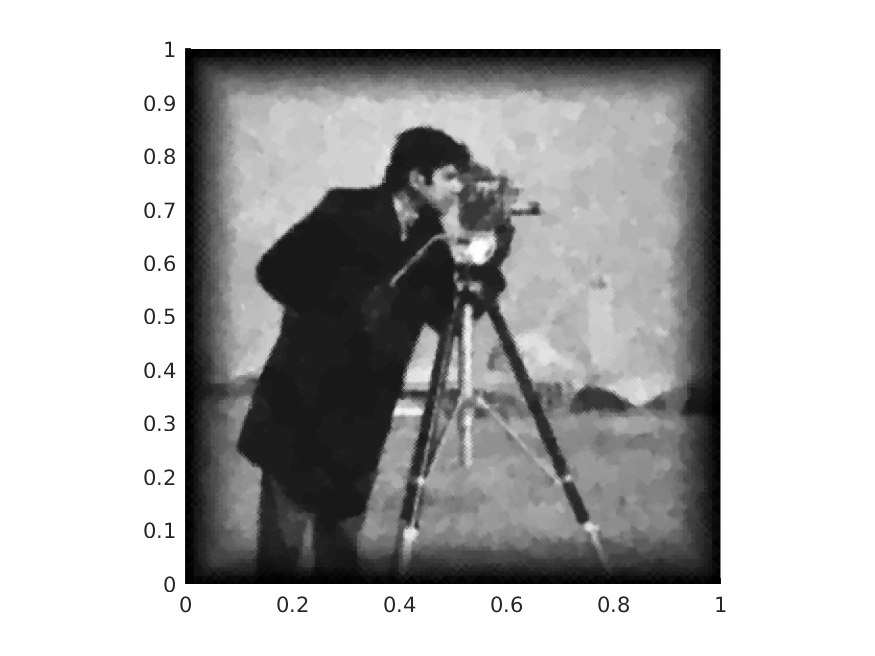
\includegraphics[trim = 60 20 60 20, clip, width=\linewidth]
      {pictures/introBeta/snr10/02500.png}
    \label{fig:snr10alpha2500}
  \end{subfigure}

  \begin{subfigure}{.3\linewidth}
    \caption{$\alpha=5000$}
    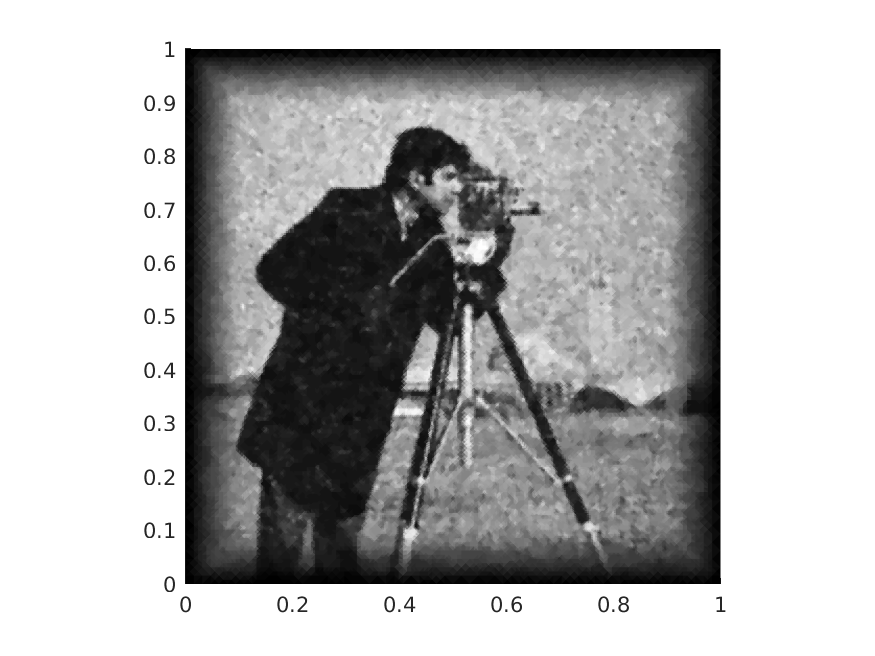
\includegraphics[trim = 60 0 60 20, clip, width=\linewidth]
      {pictures/introBeta/snr10/05000.png}
    \label{fig:snr10alpha5000}
  \end{subfigure}
  \begin{subfigure}{.3\linewidth}
    \caption{$\alpha=10000$}
    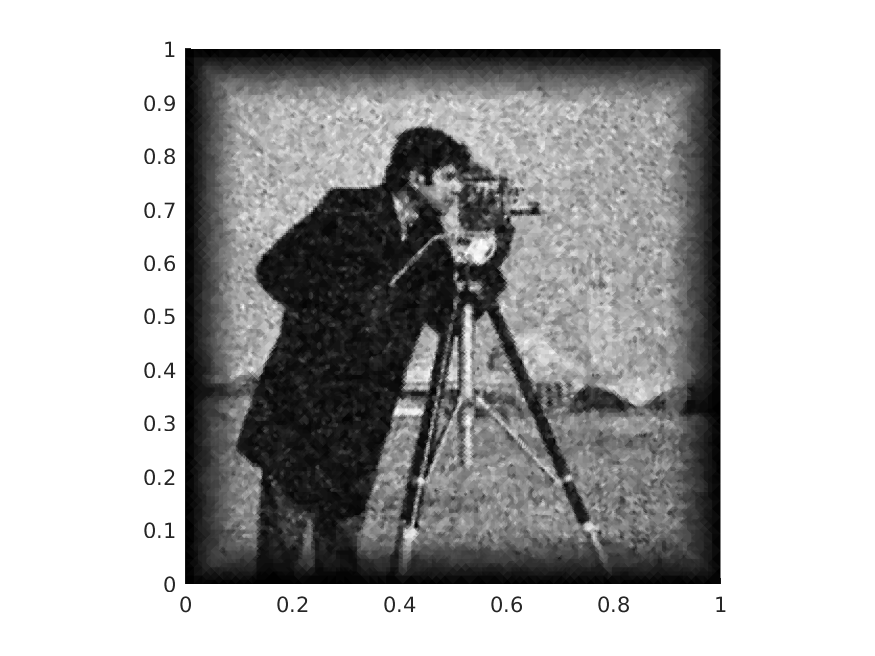
\includegraphics[trim = 60 0 60 20, clip, width=\linewidth]
      {pictures/introBeta/snr10/10000.png}
    \label{fig:snr10alpha10000}
  \end{subfigure}
  \caption{Originalbild\protect\footnotemark (a) und
    Originalbild mit additiven weißen gaußschen Rauschen (b) mit einem
    Signal-Rausch-Verhältnis (eng.\ signal-to-noise ratio, SNR) von 10, jeweils
    mit nachträglich hinzugefügten graduellen Übergang zu schwarzen Rand, um 
    Nullranddaten zu garantierten. 
    Außerdem fünf Ergebnisse (c)-(g) des in \Cref{chap:implementation}
    beschriebenen adaptiven Algorithmus mit verschiedenen Werten von $\alpha$.}
  \label{fig:exampleDenoising}
\end{figure}

\footnotetext{ 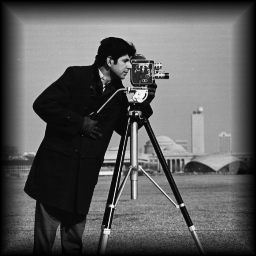
\includegraphics[height=5mm]{pictures/introBeta/cameraman.png}
\url{https://homepages.cae.wisc.edu/~ece533/images/cameraman.tif}}
